% LATER: I need a figure with some psychometric showing good performance. 
% Some cool additional analysis that would be nice to include if I have time. 
%LATER: How long does it take to learn the categorization once the initial exemplars are learned? 
%LATER: How long does it take to learn to switch after you are able to categorize? 
%LATER: How long does it take to learn the second category after you are able to learn the first? 

% Figures in this chapter
\newcommand{\Task}{1}
\newcommand{\TaskDiagram}{\Task A}
\newcommand{\TaskTrials}{\Task B}
\newcommand{\TaskSounds}{\Task C}

\newcommand{\Training}{2} 
\newcommand{\TrainingSessions}{\Training A}
\newcommand{\TrainingTrials}{\Training B}

\newcommand{\AmodEffect}{3}
\newcommand{\amodPsychometrics}{\AmodEffect A, B, D, E}
\newcommand{\amodCorrect}{\AmodEffect C, F}

\newcommand{\SingleSound}{4}
\newcommand{\SinglePsy}{\SingleSound A, C}
\newcommand{\SingleSum}{\SingleSound B, D}
\newcommand{\SingleFreqP}{\SingleSound A}
\newcommand{\SingleFreqS}{\SingleSound B}
\newcommand{\SingleAMP}{\SingleSound C}
\newcommand{\SingleAMS}{\SingleSound D}

\chapter{A behavioral task for evaluating the cortical and subcortical
contributions to sound feature discrimination}

\section{Introduction}
% We found that corticostriatal and thalamostriatal pathways send different
% information about certain sound features to the striatum. 
% DONE: Chapter number
In \ch{\Thstr}, we found that the thalamostriatal and corticostriatal
pathways send complementary information to the striatum about some features of
sound. 
%
While both pathways conveyed frequency information to the striatum with similar
fidelity, corticostriatal neurons better represented the rate of temporal
amplitude modulations in their overall spiking rate.
%
The spiking rate of thalamostriatal neurons more closely followed rapid
variations in stimulus amplitude, but the total number of spikes during the
stimulus was less indicative of the modulation rate.
% What is the significance of this difference? 
% DONE: Chapter number
While our earlier experiments in \ch{\Musc} strongly suggested a role for the
striatal target region of these projections in sound-guided behavior, the
relative contribution of these parallel pathways to behavior is unclear. 
%

% Some inactivation studies show that AM discrimination suffers after cortical
% lesions.
Lesion studies have suggested that discrimination of fast AM rates suffers
following removal of auditory cortex \citep{Deutscher2006}.
%
In contrast, sound frequency discrimination behavior has been shown to persist
after extensive lesions of AC \citep{Gimenez2015}.
%
% DONE: Phrase as either/or cortical/subcortical?
We therefore hypothesized that the cortical representation of AM is necessary
for accurate AM discrimination, but that sound frequency discrimination can be
accomplished with auditory information from the subcortex alone. 

% Specific hypothesis and test
Specifically, we hypothesized that the effect of reversible AC inactivation
would be greater on AM discrimination than on frequency discrimination. 
%
To test this hypothesis, we designed and implemented a behavioral task that
permits evaluation of the effects of a single reversible inactivation on
discriminations of both sound features.
%
We performed bilateral reversible inactivations of AC in animals trained on
this task, and found that discrimination of both features was impaired. 
%
While the contribution of the thalamostriatal and corticostriatal pathways to
discrimination of these sound features is still not clear, this task provides a
method for comparing the effect of reversible chemical manipulations on
discriminations of diverse stimulus features. 


\section{Methods}

\subsection{Animal subjects}
% DONE: Number of mice
14 adult male wild-type mice (C57/BL6J) were used in this study. Mice had ad
libitum access to food, but water was restricted. Free water was provided on
days with no experimental sessions. All procedures were carried out in
accordance with National Institutes of Health standards and were approved by
the University of Oregon Institutional Animal Care and Use Committee.

\subsection{Behavioral task}
% DONE: Update methods for amod task
Behavioral data was collected using the taskontrol platform
(\url{www.github.com/sjara/taskontrol}) developed in our laboratory using the
Python programming language (\url{www.python.org}).
%
Mice initiated each trial by poking their noses into the center port of a
three-port behavior chamber.
%
% DONE: We aren't making animals wait - check the paradigm After a silent delay
% of random duration (150-250 ms, uniformly distributed), a sound was presented
% for 500 ms.
%
The sound was either a narrow-band sound (chord), a single tone, or a
sinusoidally-amplitude-modulated white noise.
%
The decision to use chords or tones was chosen by the experimenter, and
thereafter during the behavior session the type of stimulus alternated between
cords/tones and AM sounds each trial (stimulus type was not randomized per
trial).
%
Animals were required to stay in the center port until the end of the sound and
then chose one of the two side ports for reward (2 $\mu$l of water) according
to a reward contingency that was specific to the type of sound.
%
For chords and tones, the reward contingency was: low frequency: go to left
port; high frequency: go to right port.
%
For amplitude-modulated noise, the reward contingency was: slow modulation
rate: go to left port; fast modulation rate: go to right port.
%
If animals withdrew before the end of the stimulus, the trial was aborted and
ignored in the analysis.
%
Chord stimuli were 12 simultaneous pure tones logarithmically spaced in the
range f/1.2 to 1.2f for a given center frequency f.
%
Within a behavioral session, we used 8 distinct center frequencies for chords
and tones, and 8 distinct modulation rates for AM sounds.
%
Each behavioral session lasted 60 to 90 minutes.

\subsection{Muscimol inactivation}
% DONE: Change to match muscimol protocol for amod study.  @internet
Bilateral craniotomies were performed under stereotactic surgery over the
posterior striatum (1.7 mm posterior to bregma, 3.55 mm lateral from midline)
of mice trained in the two-alternative choice sound discrimination task.
%
Headbars were implanted to allow for head-fixation.
%
Each craniotomy was protected with a plastic ring and filled with silicon elastomer (Sylgard 170, Dow Corning).
%
Animals were allowed to recover for at least 3 days before resuming behavioral training.
%
Following recovery, implanted animals were trained on the sound discrimination task until they reached their pre-surgery performance level before beginning muscimol inactivation.

For intracranial injection, we used glass pipettes (5 $\mu$l Disposable Micropipettes, VWR) pulled and trimmed to an inner diameter of 15-20 micrometers at the tip.
%
Animals were head-fixed and allowed to run on a wheel during the injection.
%
Craniotomies were exposed by removing the silicon elastomer covering, and a glass pipette filled with reagent (either muscimol or saline) was lowered into the brain to a depth of 3.1 mm from brain surface using a micromanipulator.
%
A volume of 45 nl of muscimol (0.25 mg ml$^{-1}$, final dose of 11.25 ng per bolus) was injected under air pressure in each hemisphere at a rate of 90 nl min$^{-1}$, twice per hemisphere.  %
%
One injection was given first at the front of the right craniotomy, then the front of the left craniotomy, then the rear right, and finally the rear of the left craniotomy. 
%
% Given the relationship between concentration and diffusion distance (from
% Fick's law) and previous reports of muscimol effects on neuronal activity
% \citep{Edeline2002}, we expect that by the first 10 minutes of the behavioral
% session, the effects of muscimol (50\% reduction in firing or more) will be
% confined to a volume smaller than 1 mm in diameter centered at the injection
% site. This volume matches well the extent of the posterior tail of the
% striatum (approx. 1 mm A-P, 0.6 mm M-L, 1.5 mm D-V) that receives auditory
% inputs \citep{Hunnicutt2016}.
%
The pipette was left in place for 60 seconds following each injection, then raised 0.5mm and left in place for another 60 seconds before being removed.
%
The entire injection procedure was completed within 30 minutes.
%
The craniotomies were then protected with a new silicon elastomer cap, and the mouse was placed back into its home cage for 30 minutes before starting the behavior session.
%
After collection of 4 saline sessions and 4 muscimol sessions, 45 nl of fluorescent dye (DiI, Thermo Fisher Scientific) was injected at the same injection coordinates.
%
Animals were then perfused transcardially with 5\% paraformaldehyde, and brains were extracted and postfixed for 12-24 hours.
%
Brains were then sliced (100 um) and imaged to verify the location of fluorescent dye injection.  

\subsection{Analysis of behavioral data}

% DONE: Add stuff about the GLMER models here.
Psychometric curve fitting was performed via constrained maximum likelihood to estimate the parameters of a logistic sigmoid function (\url{http://psignifit.
%
sourceforge.net}). Statistical comparisons were performed using non-parametric statistical tests with no assumption of normality. 
%
Generalized linear mixed models were fit with the R programming language (\url{https://www.r-project.org/}) using the `lme4' package (\url{http://lme4.r-forge.r-project.org/}).


\section{Results}

% DONE: Table number
We found that this task was challenging to learn, but that animals could learn to perform it well if given sufficient training time.
%
We used a set of criteria defined in Table IV.1 to determine when mice were ready to advance to the next training step.
%
Animals first advanced through a series of behavioral stages designed to familiarize them with the behavior box and begin to teach them the rules of the task.
%
During the first stage, animals received a water reward after poking their nose
in any of the three ports in the box.
%
This stage allowed animals to learn that the behavior box is a good place to
be, and engaged their natural desire to explore to teach them that they are
able to control the environment and trigger changes by poking in the ports.
%%%%%%%%

%%%%%%%%
In the next stage, animals had to poke in the center port and then go to the
side ports to collect water.
%
This stage began to teach the animals that the center port is where you go to
trigger trials, and that going to a side port is how you collect reward.
%
During these first two stages, an auditory stimulus was played to the animals when they triggered a trial by sticking their nose in the center port.
%
After animals were acquainted with the box and the idea of poking to receive water, they began to learn the sound-action association.
%
% DONE: Mention sound above
During the next stage, animals triggered a trial by poking in the center port,
and then had to go to the right port to collect a reward if the AM rate of the
presented sound was fast, and to the left port if the AM rate was slow.
%
However, on this stage animals were guided towards forming the correct
association by letting them correct their choice if they first made a mistake.
%%%%%%%%

%%%%%%%%
After animals performed well on this stage, we started requiring animals to
make a correct choice on the first try.
%
% DONE: define the range
When they were performing well on this stage, we began presenting a range of AM
rates between the previously-trained fast and slow rates (usually 8 rates,
logarithmically-spaced between the slow and fast rate used in the initial training).
%
During this stage, animals had to learn the category boundary between the
``fast'' and ``slow'' rates.
%
Once they became proficient at this discrimination, animals had good knowledge
of the task structure and rules.
%
At this point, we began to train on two narrow-band stimuli (or pure tones for
some animals).
%
We then switched to a stage where we presented a range of frequencies, logarithmically-
spaced between the initial low and high frequency, and
trained animals until they had learned the boundary between ``high'' and
``low'' sound frequencies as well.
%
% DONE: At this point is ambiguous does it mean this or the next one?
After they had been trained to categorize first AM rate, and then frequency of sound,
we started to introduce the next level of task complexity.
%%%%%%%%

%%%%%%%%
During the next training stage, the type of sound presented when animals
triggered a trial switched between an AM noise and a narrow-band chord (or pure
tone) every other trial.
%
% DONE: Takes little time to do, which is a cool feature. Talk about that here. 
The sound-action association necessary to receive reward was the same as had
been previously learned for each sound.
%
We first introduced animals to the type of sound switching by presenting only
two examples of each sound type, but then moved on to presenting a range of AM
rates and sound frequencies.
%%%%%%%%

%
% LATER: Number of sessions it took to learn the switching.
% Animals took few sessions to learn to switch back and forth between the types 
% of stimuli they were categorizing.
%%%%%%%%%%% Training structure table %%%%%%%%%%%%%%

%DONE: Last criterion to advance (to experiment ready)
After animals performed above 80\% correct on each discrimination for 3 consecutive training sessions, they were deemed ready for use in experiments. 
%
Animals took an average of 119 sessions (\fig{\TrainingSessions}) and performed an average of 100,892 trials (\fig{\TrainingTrials}) before they were deemed ready for experiments.

\begin{landscape}
% \begin{sidewaystable}
\thispagestyle{mylandscape}

\begin{table}
\resizebox{8.5in}{!}{%
\begin{tabular}{lllll}
\textbf{Stage} & \textbf{Name}        & \textbf{Goal}                           & \textbf{Water delivery}       & \textbf{Criterion to advance}              \\
SD AM          & Sides Direct, AM     & Get animals to poke and collect water   & After center or side poke     & One session with 200 rewards               \\
D AM           & Direct, AM           & Trial initiation in center poke         & After center poke             & One session with 200 rewards               \\
NC AM          & On next correct, AM  & Discover correct association            & After correct/ed side poke    & One session with 500 rewards               \\
IC AM          & If correct, AM       & Enforce correct association             & After correct side poke       & Animal performs \textgreater{}80\% correct \\
P AM           & Psychometric, AM     & Categorize AM rate                      & After correct side poke       & Animal performs \textgreater{}80\% correct \\
IC F           & If correct, Freq     & Form association for frequency          & After correct side poke       & Animal performs \textgreater{}80\% correct \\
P F            & Psychometric, Freq   & Categorize sound frequency              & After correct side poke       & Animal performs \textgreater{}80\% correct \\
IC M           & If correct, Mixed    & Switch between sound types              & After correct side poke       & Animal performs \textgreater{}80\% correct \\
P M            & Psychometric, Mixed  & Categorize both sound types             & After correct side poke       & Three sessions \textgreater{}80\% correct \\
\end{tabular}}
%DONE: Table caption (just review it one more time before nobody ever sees it again). 
\caption{Stages of behavioral shaping.}{Animals progressed through 9 behavioral training stages during behavioral shaping.
%
Each stage was designed to teach the animal a new feature of the behavioral task.
%
Animals graduated to the next phase of training when they performed above a set criterion level.
%
Over the first three training stages, animals primarily learned about the behavioral box and the structure of the task.
%
After an initial session where a nose poke in any of the three ports would trigger water, animals next had to learn to trigger rewards by poking in the center and then collecting the reward at the side.
%
The sound-action association was trained over a series of three stages, where animals could initially correct a previous incorrect response and still get a reward.
%
After this stage, a correct response was required on the first poke.
%
Once animals were capable of performing the discrimination behavior with two prototype stimuli (well-separated in stimulus space), they were then tested with a range of stimuli logarithmically-spaced between the initial two prototypes, and were required to learn the category boundary.
%
Finally, once animals were capable of categorizing both AM rate and sound frequency, the sound triggered by every nose poke began to alternate between an AM noise stimulus and a tone every other trial.
%
Animals still had to perform the previously-learned categorization on each stimulus.}
% \end{sidewaystable}
\end{table}

% \vfill
% \raisebox{-5.75in}{\makebox[\linewidth]{\thepage}}
\end{landscape}

%%%%%%%%%%%%%%%%%%%%%%%%%%%%%%%%%%%%%%%%%%%%%%%%%%%


% \subsection{Animals can switch between discriminations of different stimulus
% features every trial}
% 
% Despite the difficulty of learning this task, which was evident by the long
% time required for animals to progress through all of the many training stages,
% animals were able to achieve high levels of performance.
% NO: I need a figure with some psychometric showing good performance. 

%%%%%%%%%%%%%%%%%%%%%%%% Figure Task %%%%%%%%%%%%%%%%%%%%%%%%%%%%%
\begin{figure}[hp] \begin{center}
	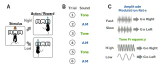
\includegraphics[width=6in]{figures/chapter4/figure_task} \end{center}
	\caption{A behavioral task for evaluating the effects of reversible
	inactivation on discrimination of different sound
	features.}{\textbf{(A)} Schematic of the two-alternative choice sound
	feature discrimination task. Mice initiated each trial by entering a
	center port and had to choose one of two side reward ports depending on
	the sound presented.
	%
\textbf{(B)} The type of sound presented was alternated every other trial. 
%
% DONE: Make sure all other figure captions have bold cap labels
\textbf{(C)} On trials when an AM noise stimulus was presented, mice had to
choose the right reward port if the modulation rate was fast and the left
reward port if the modulation rate was slow to be rewarded. On trials when a
narrow band chord was presented, mice were rewarded for picking the right port
if the sound frequency was high and the left port if the sound frequency was
low. 
%
}
\end{figure}
%%%%%%%%%%%%%%%%%%%%%%%%%%%%%%%%%%%%%%%%%%%%%%%%%%%%%%%%%%%%%%%%%%%%%

% DONE: I think this figure should come earlier. 
%%%%%%%%%%%%%%%%%%%%%%%% Figure Training Time %%%%%%%%%%%%%%%%%%%%%%%%%%%%%
\begin{figure}[hp] \begin{center}
	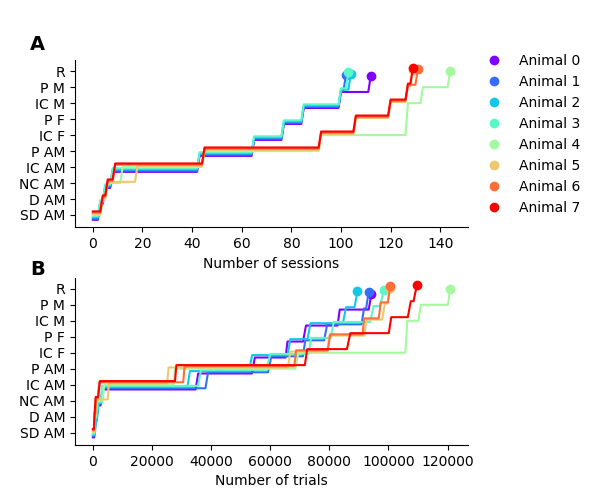
\includegraphics[width=6in]{figures/chapter4/figure_training}%
\end{center} \caption{Animals took about 4 months to learn the
task.}{\textbf{(A)} Animals progressed through 9 training steps over an average
of 119 behavioral training sessions before being ready for experiments (min:
102 sessions; max: 144 sessions). 
%
\textbf{(B)} Animals performed an average of 100,892 trials before being ready
for experiments (min: 89,527; max: 120,885). 
%
} \end{figure}
%%%%%%%%%%%%%%%%%%%%%%%%%%%%%%%%%%%%%%%%%%%%%%%%%%%%%%%%%%%%%%%%%%%%%

\subsection{Reversible inactivation of AC affects discrimination of both sound
frequency and AM rate}

After animals had learned the task, we began performing
bilateral intracranial injections of either the GABA agonist muscimol, or a
saline control, 30 minutes before each behavioral sessions.
%
We alternated between muscimol and saline injections each day. 
%
Muscimol injection affected performance on both tone and AM trials, resulting
in both a flattening of the psychometric curve (\fig{\amodPsychometrics}) and a
reduction in overall performance (\fig{\amodCorrect}) for both animals tested. 
%
We tested the hypothesis that muscimol has a stronger effect on AM
discrimination performance than on frequency discrimination performance by
comparing two generalized linear mixed effect regression models, both attempting
to explain the variance in correct response likelihood that was explained by the
identity of the injection (saline \emph{vs.} muscimol). 
%
In the null model, we allowed the intercept to differ between data from the two
sound types.
%
This inclusion of a random intercept for different sound types helped to account for the fact that animals often performed much better on the
frequency discrimination trials than on AM discrimination trials.
%
Against this null model we compared a model which allowed both random
intercept for sound type, allowing for the fact that performance started
at a different level, as well as allowing for random slopes (a difference in
the strength of the effect between the two sound types).
%
For both models we additionally allowed the slope and intercept of the muscimol
effect to vary between the animals included in the comparison (n=2). 
%
Allowing for random slopes of the effect of muscimol based on sound type did
not significantly increase the variance explained by the model
($\chi^{2}$=1.64, p=0.44).
%
Therefore, we fail to reject the null hypothesis that the strength of the
muscimol effect is the same for discrimination of frequency and AM rate. 

% Inactivation caused deficits in discrimination of both types of stimuli.
\begin{figure}[hp] \begin{center}
    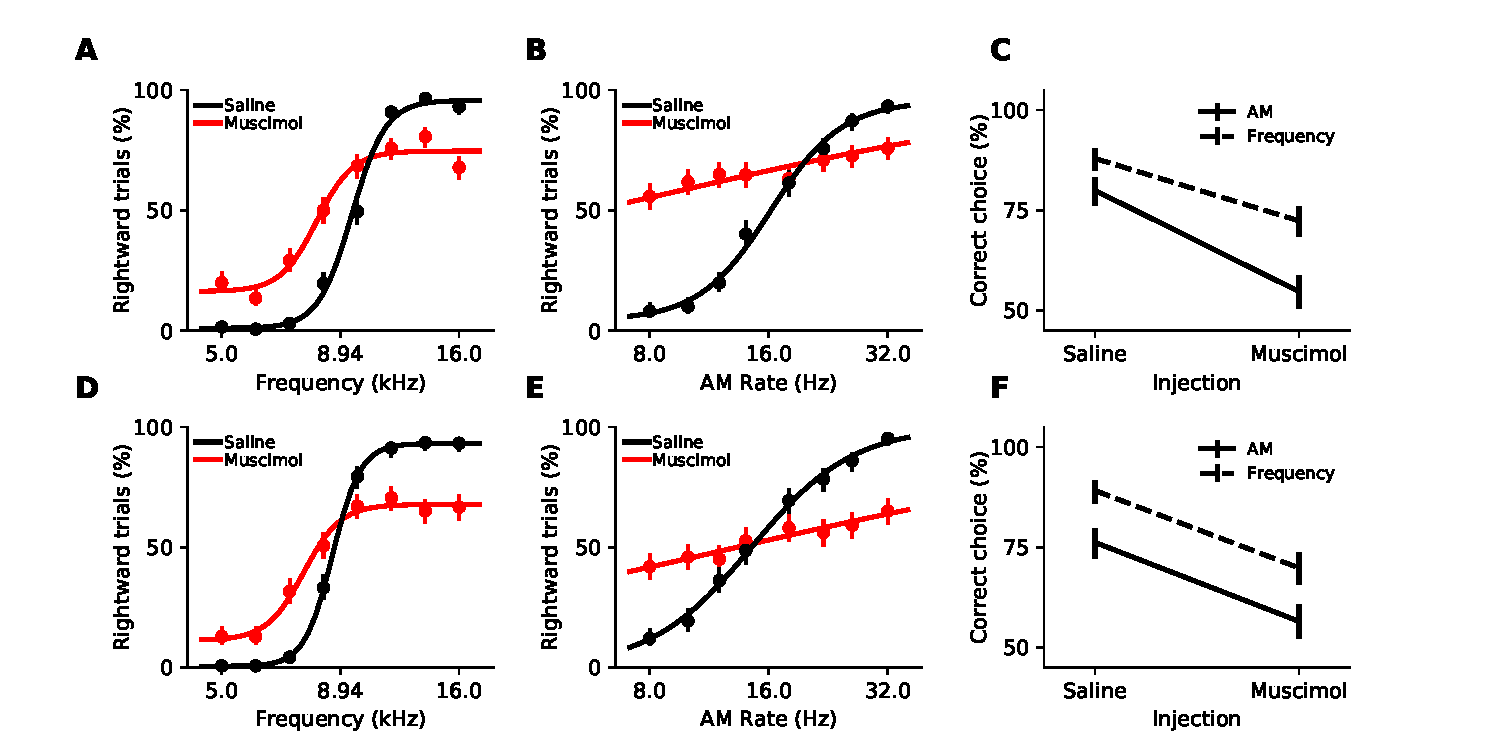
\includegraphics[width=6in]{figures/chapter4/figure_main_amod_effect}%
\end{center} \caption{Reversible inactivation of AC impairs both frequency and
AM discrimination.}{ \textbf{(A)} Frequency discrimination psychometric
performance for subject 1, averaged over 5 saline sessions (black points) and 5
muscimol sessions (red points).
%
\textbf{(B)} AM discrimination psychometric performance for subject 1, averaged
over 5 saline sessions (black points) and 5 muscimol sessions (red points). 
%
\textbf{(C)} Average percent correct for subject 1, averaged over 5 saline
sessions and 5 muscimol sessions.
%
Dotted line indicates the effect of muscimol injection on sound frequency
discrimination performance. 
%
Solid line indicates the effect of muscimol injection on AM rate discrimination
performance.
%
Error bars indicate 95\% binomial proportion confidence intervals.
%
\textbf{(D, E, F)} Same as A, B, and C, respectively, for subject 2.  }
\end{figure}
% 
% % The effect of inactivation is not different between the two stimuli (GLMER
% % results).
% 
% \subsection{AC inactivation affects discrimination of both features when during
% sessions with a single sound type}
% % DONE: Did they learn both, and then get transferred to 2? Was it the same
% % between?
% For a subset of animals, we performed reversible inactivation of AC during
% sessions where subjects only had to discriminate a single sound type.
% %
% Under these conditions, we still observed an effect of muscimol both on
% psychometric performance (\textbf{\fig{\SinglePsy}}) and on overall percent
% correct (\textbf{\fig{\SingleSum}}).
% 
% % We have a few sessions where we show that both discriminations are hurt
% % individually, arguing against the idea that the cortically-dependent part of
% % the task is the switching. 
% 
% %%%%%%%%%%%%%%%%%%%%%%%% Figure Single Sound Type %%%%%%%%%%%%%%%%%%%%%%%%%%%%%
% \begin{figure}[hp] \begin{center}
%     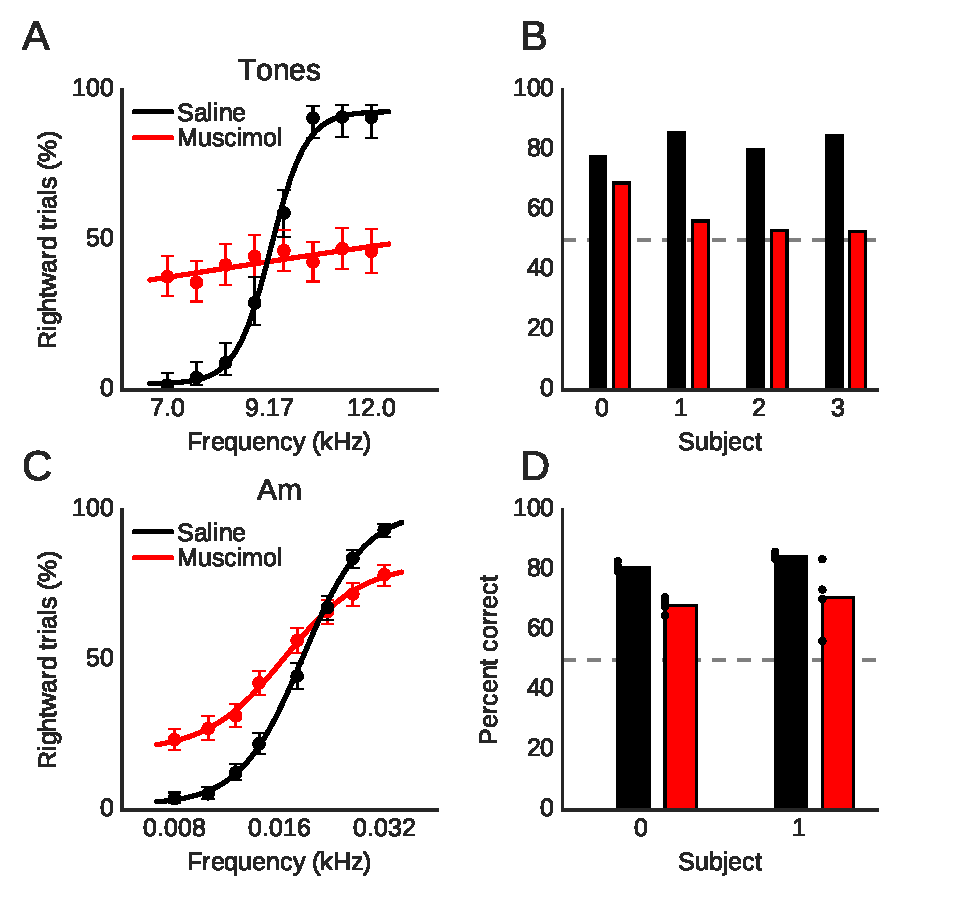
\includegraphics[width=6in]{figures/chapter4/figure_single_sound_type}%
% \end{center} \caption{Muscimol affects each discrimination when performed
% independently.}{\textbf{(A)}  Example psychometric curve from sessions where an
% animal discriminated only high sound frequency from low sound frequency.
% Performance suffers in sessions where muscimol was injected in AC (red, 1
% session) compared to control saline injection (black, 1 session).
% % DONE: How to have number of sessions here? 
% %
% \textbf{(B)} Average percent correct for 4 animals during muscimol (red, 1
% session per animal) and saline (black, 1 session per animal) sessions. 
% %
% \textbf{(C)} Example psychometric curve from sessions where an animal
% discriminated only fast AM rates from slow AM rates. Performance suffers in
% sessions where muscimol was injected in AC (red, 4 sessions) compared to
% control saline injection (black, 4 sessions).
% %
% \textbf{(D)} Average percent correct for 2 animals during muscimol (red, 4
% sessions per animal) and saline (black, 4 sessions per animal) sessions.  }
% \end{figure}


\section{Discussion}

This behavioral paradigm was designed to facilitate comparison of the same manipulation of neural activity on discrimination of two different sound features, in order to address the question: Is auditory cortex required for discrimination of some sound features, while discrimination of other sound features can be accomplished with subcortical pathways alone? 
%
We found that animals were able to learn the task, although it took a long time to train them to perform it at a high degree of accuracy. 
%
We performed reversible inactivation of auditory cortex in two animals trained in this task, and observed deficits in both frequency and AM discrimination. 
%
Future experiments must leverage the flexibility of the 2AFC paradigm, by manipulating the stimulus sets presented, to bring the psychometric performance for each sound type to the same starting point before performing inactivations. 
%
Importantly, we chose to use reversible inactivation with muscimol in this study for several reasons, but this behavioral paradigm can generalize to other inactivation techniques as well. 
%
It is likely that a full picture of the role of sensory cortex in the two discriminations tested would rely on information gained from inactivation experiments with different methods of manipulating or silencing activity. 

\subsection{Information from reversible inactivation vs. lesion experiments}
% What is the role of chemical inactivations when you could just do lesions so that you know the exact boundary of the removed tissue?
Lesions have the advantage of allowing precise histological determination of the regions that are removed or damaged. 
%
% NO : Refs
Lesions can also lead to different results than transient inactivations, an effect often assumed to be related to compensatory plasticity occurring after the lesion and before the behavioral assessment. 
%
However, the comparison of both lesion and transient inactivation experiments can lead to a fuller picture of the role of a brain area in a behavior. 
%
If a downstream region receives connections from both a cortical and a subcortical area, then transient inactivation of the cortical region could lead to unbalanced inputs in the downstream region and cause task deficits, even if the cortical representation of the information isn't any more useful for solving the behavioral task than the subcortical representations. 
%
Following a lesion of the cortical region, the downstream area could undergo homeostatic rebalancing of its inputs, and the discrimination could be solved again using only the input from the subcortical pathway. 
%
In this situation, the lesion study alone may lead to the erroneous conclusion that the cortical region is not at all involved in task performance under normal circumstances, and the transient inactivation experiment would lead to the erroneous conclusion that the information from the subcortical pathway is not sufficient, or at least less useful, for solving the discrimination task. 
%%%%%%%%

%%%%%%%%
A more nuanced way of examining the role of brain regions is laid out in \citet{Otchy2015}. 
%
The authors argue that brain areas should be categorized as \emph{necessary} or \emph{permissive} for task performance by using a combination of both lesion and transient inactivation experiments. 
%
An area is \emph{permissive} for task performance if it is involved in task performance under normal conditions, but doesn't provide any information that can't be obtained from other pathways or areas. 
%
Transient inactivation of a permissive structure will cause deficits in task performance, but lesion of the area, with a recovery period afterward to allow downstream areas to adapt to changes in their inputs, would not.
%
An area that is truly \emph{necessary} provides information that cannot be obtained from another source. 
%
Thus, performance would still suffer after lesion, even if you allow a period for downstream circuits to adapt.

\subsection{What did we learn from preliminary inactivations?}
We performed inactivations over many behavioral sessions in two trained animals, showing that this method allows us to resolve the effect of the manipulations on discrimination of each sound type. 
%
However, interpretation was hampered by the fact that pre-inactivation performance was not equivalent between the two sound types. 
%
Therefore, it was not clear whether a decrease from 85\% correct to 75\% correct and decrease from 75\% correct to 65\% correct were effects of equivalent magnitude. 
% 
Future experiments should carefully match pre-inactivation performance between the sound types for each animal by adjusting the range of sounds presented during the psychometric sessions.
%
Nevertheless, it was clear from these inactivation experiments that there was an effect of cortical inactivation on discrimination of both sound types, and that evaluation of the relative necessity of sensory cortex for performing two discrimination of two different sound features will require precise comparison of the magnitude of the effect on each discrimination.

\section{Link to Chapter V}
In this chapter, we present a behavioral task for evaluating the effect of chemical inactivation of auditory cortex on frequency and AM rate discrimination performance. 
%
% DONE: Change this to highlight the results less. 
This behavioral paradigm provides a platform for evaluating the effect of a manipulation of neural activity on discrimination of two different stimuli, in order to address the question: Is the information provided by sensory cortex to downstream areas necessary for discrimination of some types of sounds, while discrimination of other sound types can be performed using information from subcortical pathways alone?
%
In the next chapter, we expand from considering just the role of auditory cortex in the context of this task, to examine the role of other sensory cortical regions in different tasks requiring animals to make flexible associations between stimuli and actions. 

